\chapter{Solides Geld}
\label{les:14}

\begin{chapquote}{Lewis Carroll, \textit{Alice im Wunderland}}
\enquote{Das erste, was ich zu tun habe,} sagte sich Alice, als sie in dem Wald
umherwanderte, \enquote{ist meine richtige Größe wiederzuerlangen; und das
zweite ist, den Weg in den prächtigen Garten zu finden. Ich glaube, das ist der
beste Plan.}
\end{chapquote}

Die wichtigste Lektion die ich von Bitcoin gelernt habe ist, dass auf lange
Sicht hartes Geld dem weichen Geld überlegen ist. Hartgeld, auch als
\enquote{\textit{sound money}} (solides oder gesundes Geld) bezeichnet, ist eine
weltweit gehandelte Währung die als zuverlässiger Wertspeicher dient.

Zugegeben, Bitcoin ist heute noch jung und volatil. Kritiker werden anführen,
dass es nicht sonderlich zuverlässig einen Wert speichert. Das Argument mit der
Volatilität geht jedoch am Thema vorbei. Es ist natürlich mit Volatilität zu
rechnen. Der Markt wird eine Weile brauchen um den gerechten Preis für dieses
neue Geld herauszufinden. Außerdem ist die Volatilität, wie oft scherzhaft
hervorgehoben wird, auf einen Messfehler zurückzuführen. Wenn du in Dollar
denkst wirst du daran scheitern zu erkennen, dass ein Bitcoin immer ein Bitcoin
bleiben wird.

\begin{quotation}\begin{samepage}
\enquote{Eine feste Geldmenge oder eine Menge, die nur nach objektiven und
berechenbaren Kriterien verändert wird, ist eine notwendige Bedingung für einen
sinnvollen und gerechten Geldpreis.}
\begin{flushright} -- Fr. Bernard W. Dempsey, S.J.\footnote{Perry J. Roets, S.J., \textit{Review of Social Economy} \cite{review-social-economy}}
\end{flushright}\end{samepage}\end{quotation}

Wie ein kurzer Spaziergang durch den Friedhof der vergessenen Währungen gezeigt
hat: Sobald die Möglichkeit besteht Geld zu drucken, wird auch Geld gedruckt.
Bisher war kein Mensch in der Lage dieser Versuchung zu widerstehen.

Bitcoin beseitigt die Versuchung Geld zu drucken auf geniale Weise. Satoshi war
sich unserer Gier und Fehlbarkeit bewusst --- deshalb wählte er etwas weitaus
zuverlässigeres als die menschliche Zurückhaltung: Die Mathematik.

\begin{center}
  \centering
  \begin{equation}
  \sum\limits_{i=0}^{32} \frac{21000 \lfloor \frac{50*10^8}{2^i} \rfloor}{10^8}
  \end{equation}
  \caption{Die Formel für die Angebotsmenge von Bitcoin}
  \label{fig:supply-formula-white}
\end{center}

Die Formel in Abbildung~\ref{fig:supply-formula-white} ist zwar nützlich um das
Angebot von Bitcoin zu beschreiben, sie ist aber im Code eigentlich nirgendwo zu
finden. Die Ausgabe neuer Bitcoins ist algorithmisch gesteuert, da sich die
Vergütung, die den Minern als Belohnung bezahlt wird, alle vier Jahre
halbiert~\cite{btcwiki:supply}. Die obige Formel wird verwendet um diesen
Mechanismus mathematisch zu beschreiben. Was wirklich passiert lässt sich am
besten an der Veränderung der Höhe der Belohnung pro Block ablesen. Jener
Belohnung die dem Finder eines gültigen Blocks ausgezahlt wird, was etwa alle zehn
Minuten geschieht.

\begin{center}
  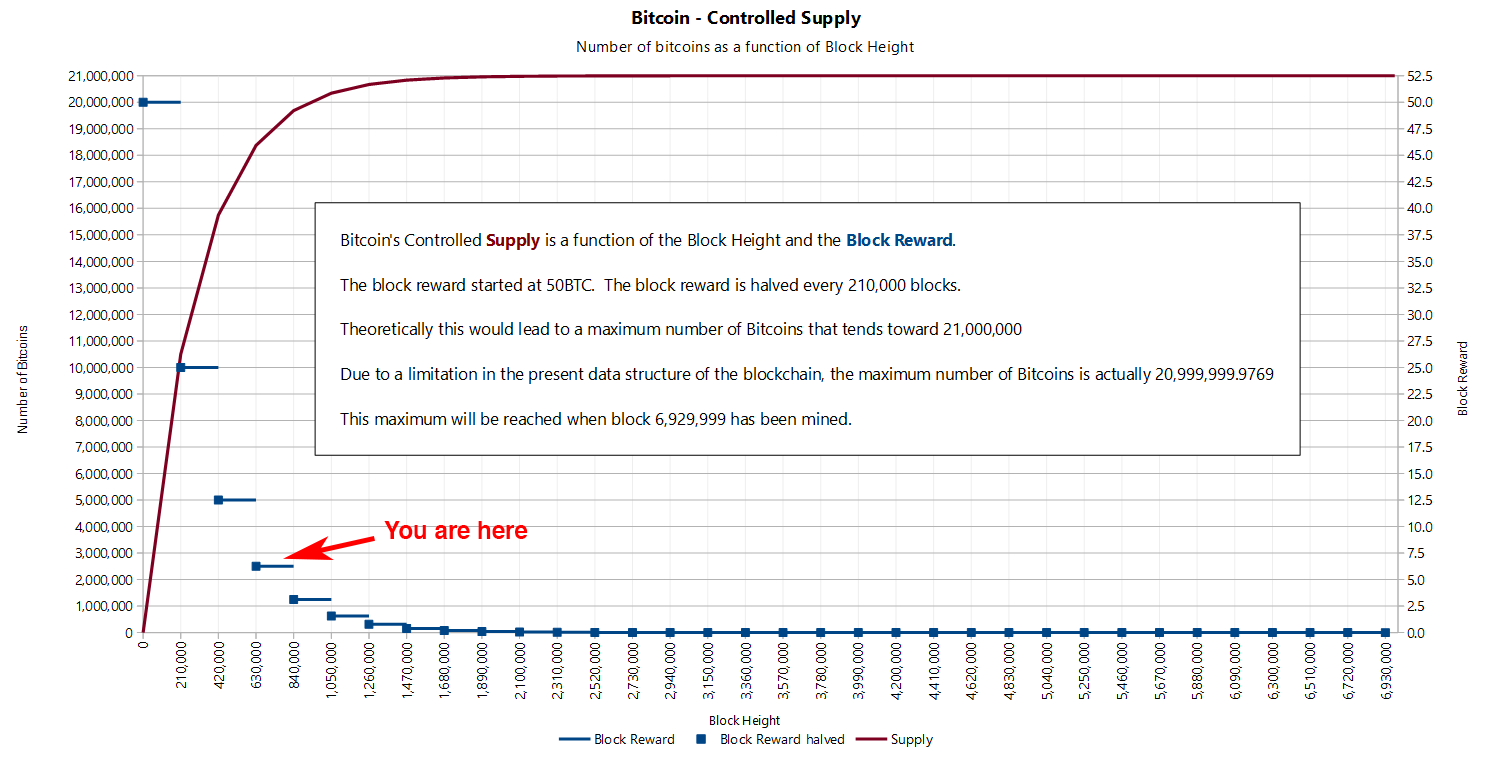
\includegraphics[width=\textwidth]{assets/images/you-are-here.png}
  \caption{Die kontrollierte Ausschüttung von Bitcoin}
  \label{fig:you-are-here.png}
\end{center}

Formeln, logarithmische Funktionen und exponentielle Kurven sind nicht gerade
intuitiv zu verstehen. Der Begriff der Solidität (\textit{\enquote{soundness}})
ist leichter zu verstehen, wenn man ihn anders betrachtet. Sobald wir wissen, wie
viel es von etwas gibt, und sobald wir wissen, wie schwer es ist dieses Gut
herzustellen (oder in die Hände zu bekommen) verstehen wir relativ schnell den
Wert dieses Gutes. Was für Picassos Gemälde, Elvis Presleys Gitarren und
Stradivari-Geigen gilt, gilt auch für Papiergeld, Gold und Bitcoins.

Die Härte des Fiatgeldes hängt davon ab, wer für den Betrieb der jeweiligen
Druckmaschinen verantwortlich ist. Manche Regierungen sind bereit große Mengen
an Währung zu drucken, was zu einer schwächeren Währung führt. Andere
Regierungen sind eher zurückhaltend beim Geld drucken, was zu einer härteren
Währung führt.

\begin{samepage}\begin{quotation}
\enquote{Ein wichtiger Aspekt dieser neuen Realität ist, dass Institutionen wie
die Fed nicht bankrott gehen können. Sie können jeden Geldbetrag drucken den sie
für sich selbst benötigen, praktisch ohne Kosten.}
\begin{flushright} -- Jörg Guido Hülsmann\footnote{Jörg Guido Hülsmann, \textit{The
Ethics of Money Production}~\cite{hulsmann2008ethics}}
\end{flushright}\end{quotation}\end{samepage}

Bevor wir Fiatgeld hatten, wurde die \enquote{\textit{soundness}} (Solidität)
des Geldes durch die natürlichen Eigenschaften des Materials bestimmt, welches
wir als Geld verwendeten. Die Menge an Gold auf der Erde ist durch die Gesetze
der Physik begrenzt. Gold ist selten weil Supernovas und
Neutronensternkollisionen selten sind. Der \enquote{Fluss} des Goldes ist
begrenzt, da die Gewinnung des Gutes sehr aufwendig ist. Als schweres Element
ist es meist tief unter der Erde vergraben.

Die Abschaffung des Goldstandards ebnete den Weg zu einer neuen Realität: Das
Hinzufügen von neuem Geld erfordert nur einen Tropfen Tinte. In unserer heutigen
modernen Welt erfordert das Hinzufügen von ein paar Nullen zum Saldo eines
Bankkontos noch viel weniger Aufwand: Ein paar Bits die auf einem Bankencomputer
geändert werden.

Das oben skizzierte Prinzip lässt sich allgemeiner als das Verhältnis von
\enquote{\textit{Stock}} zu \enquote{\textit{Flow}} (Bestand zu Zufluss)
ausdrücken. Einfach ausgedrückt ist der \textit{Stock} (Bestand), wie viel von
etwas derzeit vorhanden ist. Für unsere Zwecke ist der Bestand ein Maß für die
aktuelle Geldmenge. Der \textit{Flow} (Zufluss) ist die Menge die über einen
bestimmten Zeitraum (z.B. pro Jahr) produziert wird. Der Schlüssel zum
Verständnis von solidem Geld (\textit{sound money}) liegt im Verständnis dieses
Stock-to-Flow-Verhältnisses.

Die Berechnung eines Stock-to-Flow Verhältnisses für ein Fiatgeld ist schwierig,
denn wie viel Geld es gibt hängt davon ab welche Zahlen man
betrachtet~\cite{wiki:money-supply}. Man könnte nur Banknoten und Münzen (M0)
zählen, Bargeld und Ersparnisse mit sofortiger Zugriffsmöglichkeit (M1)
hinzufügen, Ersparnisse und Geldeinlagen mit zweijähriger Laufzeit (M2) hinzufügen
und sogar alle Schulden und Wertpapiere mit hinzufügen (M3). Darüber hinaus ist
die Definition und Messung all dessen von Land zu Land unterschiedlich. Da die
US-Notenbank die Veröffentlichung von Zahlen für M3 eingestellt hat
\cite{web:fed-m3}, werden wir uns mit dem Geldmengenangebot M2 begnügen müssen.
Ich würde diese Zahlen ja gerne überprüfen, aber ich schätze wir müssen der
Fed vorerst vertrauen.

Gold, eines der seltensten Metalle der Erde hat das höchste
Stock-to-Flow-Verhältnis. Nach Angaben der \textit{US Geological Survey} wurden
insgesamt etwas mehr als 190.000 Tonnen abgebaut. In den letzten Jahren wurden
rund 3.100 Tonnen Gold pro Jahr gefördert.~\cite{mineral-commodity-summaries}

Mit diesen Zahlen können wir das Stock-to-Flow-Verhältnis für Gold leicht
berechnen (siehe Abbildung~\ref{fig:stock-to-flow-gold}).

\begin{center}
  \centering
  \begin{equation}
  \frac{190,000 t}{3,100 t} = ~ 61
  \end{equation}
  \caption{Stock-to-Flow Verhältnis von Gold}
  \label{fig:stock-to-flow-gold}
\end{center}

Nichts hat ein höheres Stock-to-Flow-Verhältnis als Gold. Deshalb war Gold
bisher das härteste und zuverlässigste Geld das es gab. Es wird oft behauptet,
dass das gesamte bisher geförderte Gold in zwei Olypmia Schwimmbecken passen
würde. Nach meinen Berechnungen\footnote{\url{https://bit.ly/gold-pools}} würden
wir vier brauchen. Vielleicht sollte das aktualisiert werden oder aber die
olympischen Schwimmbäder werden kleiner.

Nun zu Bitcoin. Wie du wahrscheinlich weißt, war das Bitcoin-Mining in den
letzten Jahren ziemlich im Trend. Denn wir befinden uns noch in den Anfängen der
so genannten \textit{Belohnungs-Ära}, in der Miner mit verhältnismäßig vielen
Bitcoins für ihren Rechenaufwand belohnt werden. Wir befinden uns derzeit in der
Belohnungsära Nummer 3, die 2016 begann und Anfang 2020 (wahrscheinlich im Mai)
enden wird. Während die Bitcoin-Geldmenge vorgegeben ist, erlauben die inneren
Mechanismen nur die ungefähre Vorhersage des Tages X der Halbierung. Dennoch
können wir mit Sicherheit vorhersagen wie hoch das Stock-to-Flow-Verhältnis von
Bitcoin sein wird. Spoiler-Alarm: Es wird hoch sein.

Wie hoch? Nun es stellt sich heraus, dass Bitcoin unendlich hart werden wird
(siehe Abbildung~\ref{fig:stock-to-flow-white-cropped}).

\begin{center}
  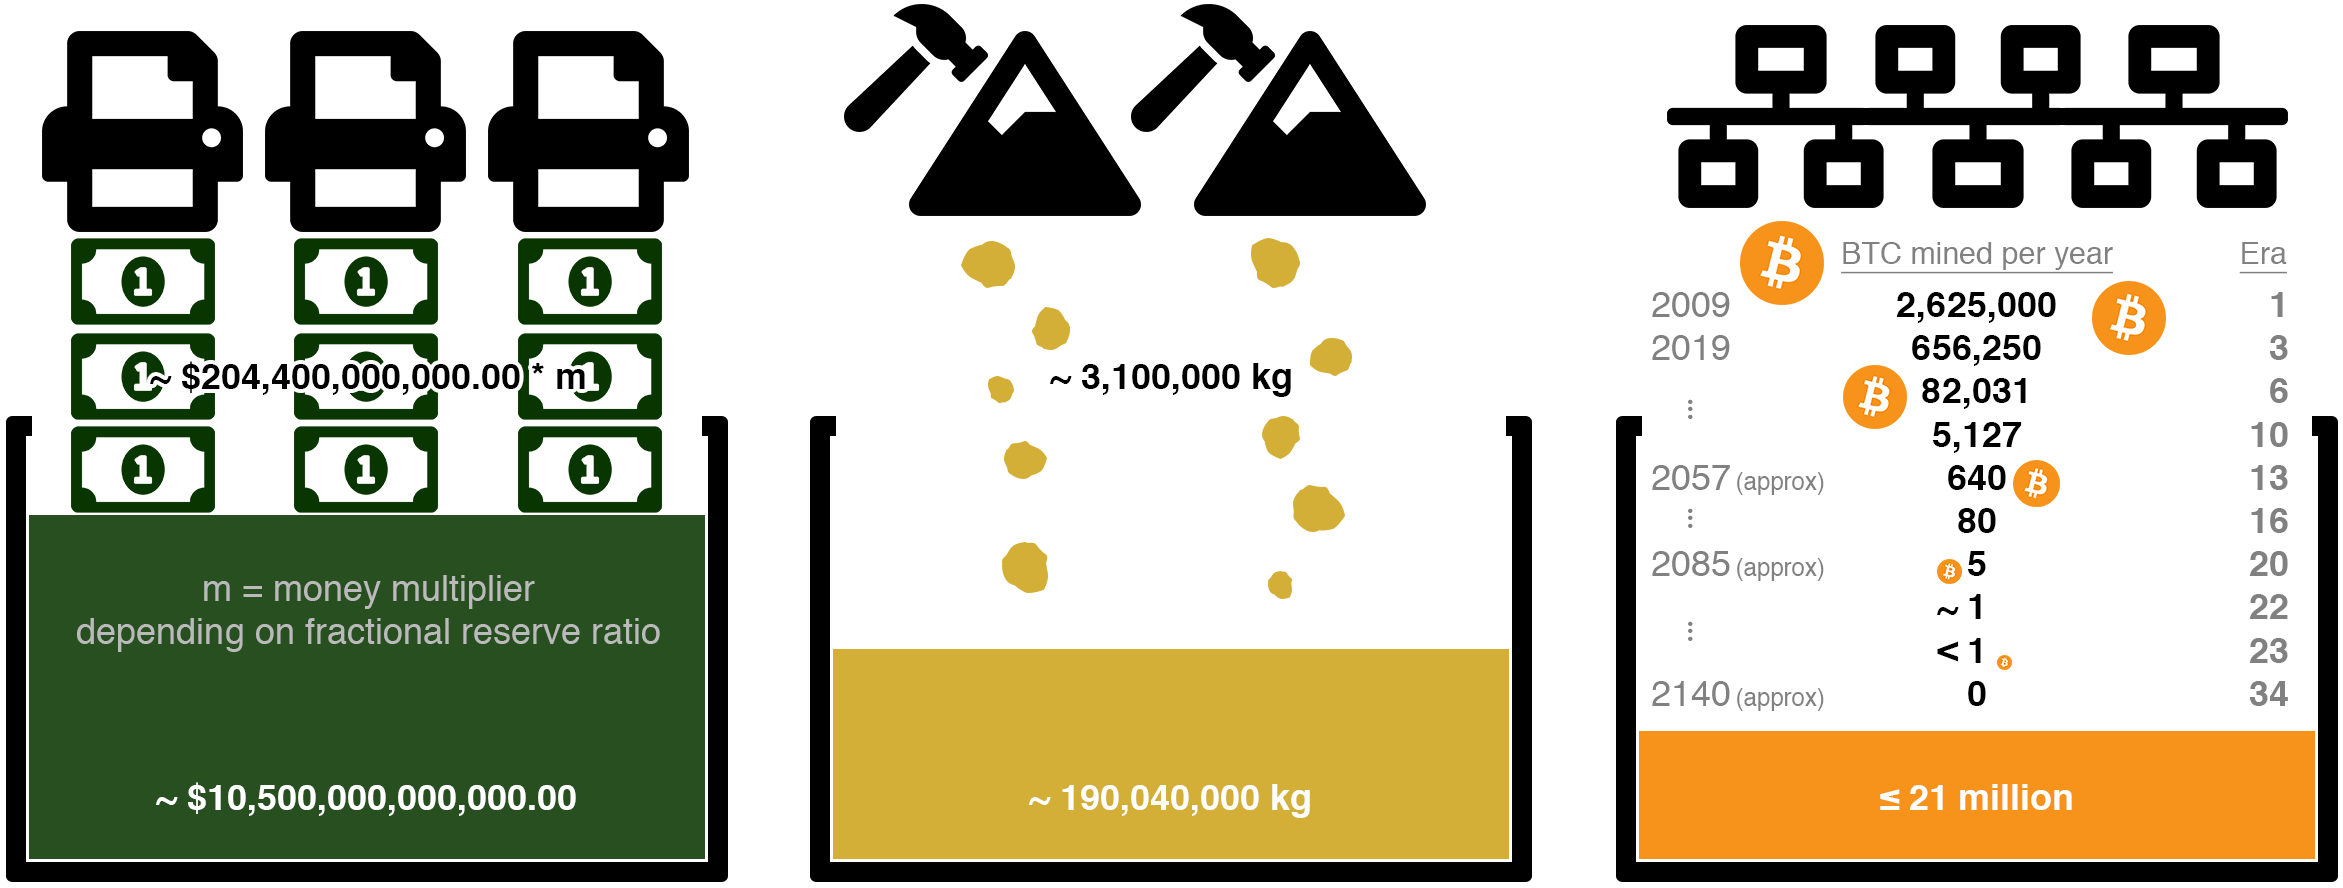
\includegraphics[width=\textwidth]{assets/images/stock-to-flow-white-cropped.png}
  \caption{Die Visualisierung des Stock-to Flow Modells für Fiat, Gold und Bitcoin}
  \label{fig:stock-to-flow-white-cropped}
\end{center}

\paragraph{}
Der Zufluss an neuen Bitcoins wird aufgrund der exponentiellen Abnahme der
Mining Belohnungen rapide abnehmen. Dies führt zu einem stark ansteigendem
\textit{Stock-to-Flow}-Verhältnis. Im Jahr 2020 wird das S2F-Verhältnis von Bitcoin
zu dem von Gold aufschließen und vier Jahre später wird es das von Gold übertreffen. Es
verdoppelt seine \enquote{\textit{soundness}}. Diese Verdoppelung wird insgesamt
64 Mal stattfinden. Da dies ein exponentieller Trend ist, wird die Zahl der
jährlich abgebauten Bitcoins in 50 Jahren unter 100 und in 75 Jahren
unter einen Bitcoin sinken. Die globale Frischversorgung an Bitcoin, den die
Blockbelohnung darstellt, wird irgendwann um das Jahr 2140 versiegen und die
Quelle von neuen Bitcoins wird versiegen. Das ist ein sehr langer Zeitraum. Wenn
du das liest bist du wahrscheinlich noch sehr früh dran.

\begin{center}
  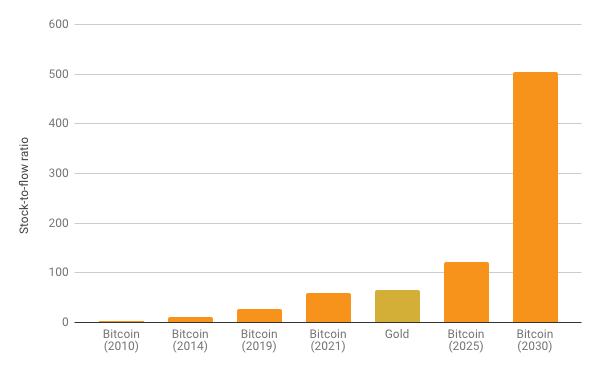
\includegraphics[width=\textwidth]{assets/images/soundness-over-time.png}
  \caption{Steigendes Stock-to-Flow-Verhältnis von Bitcoin im Vergleich zu Gold}
  \label{fig:soundness-over-time}
\end{center}

Je weiter sich Bitcoin dem unendlich steigenden Stock-to-Flow Verhältnis
annähert, umso solider wird es. Unendliche \enquote{soundness} ist schwer zu
übertreffen.

Aus der Sicht der Ökonomie ist die Schwierigkeitsanpassung
(\textit{difficulty-adjustment}) von Bitcoin wahrscheinlich die wichtigste
Komponente des Systems. Wie schwer es ist Bitcoin zu schürfen hängt davon ab,
wie schnell neue Bitcoins abgebaut werden\footnote{Es hängt eigentlich davon ab,
wie schnell gültige Blöcke gefunden werden, aber für unsere Zwecke ist dies
dasselbe wie \enquote{Bitcoins zu schürfen} und das wird auch für die nächsten
120 Jahre so bleiben.}. Es ist die dynamische Schwierigkeitsanpassung, die es
uns ermöglicht die zukünftige Geldmenge vorherzusagen.

Die Einfachheit des Algorithmus der Schwierigkeitsanpassung mag von seiner
Bedeutung  ablenken, aber der Mechanismus der Schwierigkeitsanpassung ist
wirklich eine Revolution von einsteinischem Ausmaße. Er stellt sicher, dass
die vorbestimmte Geldmenge von Bitcoin nicht beeinflusst wird, unabhängig davon
wie viel oder wie wenig Aufwand für den Abbau aufgewendet wird. Im Gegensatz zu
jeder anderen Ressource, egal wie viel Energie jemand in den Abbau von Bitcoin
steckt, die Gesamtvergütung wird nicht steigen.

So wie $E=mc^2$ die Lichtgeschwindigkeit und damit das absolute
Geschwindigkeitslimit in unserem Universum vorgibt, so bestimmt die
Schwierigkeitsanpassung von Bitcoin das \textit{universelle Geldlimit} im
Bitcoin System.

\paragraph{}
Ohne die Schwierigkeitsanpassung wären alle Bitcoins bereits abgebaut worden.
Bitcoin hätte seine Kindertage ohne die Schwierigkeitsanpassung wahrscheinlich
nicht überlebt. Die Schwierigkeitsanpassung sichert das Netzwerk in seiner
Belohnungs-Ära ab und gewährleistet eine gleichmäßige und faire
Verteilung\footnote{Dan Held, \textit{Bitcoin's Distribution was
Fair}~\cite{distribution-was-fair}} von neuen Bitcoins. Sie ist das Thermostat,
welches die Geldpolitik von Bitcoin regelt.

Einstein offenbarte uns eine neue Erkenntnis: Egal wie stark man ein Objekt auch
beschleunigt, ab einem gewissen Punkt wird man nicht mehr Geschwindigkeit
herausholen können. Satoshi zeigte uns auch etwas Neues: Egal wie sehr man nach
diesem digitalen Gold graben möchte, ab einem gewissen Punkt wird man nicht mehr
Bitcoin herausholen können. Zum ersten Mal in der Geschichte der Menschheit
haben wir ein monetäres Gut von dem man --- egal wie sehr man es versucht ---
nicht mehr produzieren kann.

\paragraph{Bitcoin lehrte mich, dass solides Geld unerlässlich ist.}

% ---
%
% #### Through the Looking-Glass
%
% - [Bitcoin's Energy Consumption: A Shift in Perspective][much energy]
%
% #### Down the Rabbit Hole
%
% - [The Ethics of Money Production][Jörg Guido Hülsmann] by Jörg Guido Hülsmann
% - [Mineral Commodity Summaries 2019][last few years] by the United States Geological Survey
% - [Bitcoin’s Distribution was Fair][fair distribution] by Dan Held
% - [Bitcoin's Controlled Supply][algorithmically controlled] on the Bitcoin Wiki
% - [Money Supply][how much money there is], [Speed of Light][universal speed limit] on Wikipedia
%
% <!-- Internal -->
% [much energy]: 
%
% [Fr. Bernard W. Dempsey, S.J.]: https://www.jstor.org/stable/29769582
% [Jörg Guido Hülsmann]: https://mises.org/sites/default/files/The%20Ethics%20of%20Money%20Production_2.pdf
% [stopped publishing]: https://www.federalreserve.gov/Releases/h6/discm3.htm
% [last few years]: https://minerals.usgs.gov/minerals/pubs/mcs/2018/mcs2018.pdf
% [my calculations]: https://www.wolframalpha.com/input/?i=volume+of+190000+metric+tons+gold+%2F+olympic+swimming+pool+volume
% [fair distribution]: https://blog.picks.co/bitcoins-distribution-was-fair-e2ef7bbbc892
%
% <!-- Bitcoin Wiki -->
% [algorithmically controlled]: https://en.bitcoin.it/wiki/Controlled_supply
%
% <!-- Wikipedia -->
% [how much money there is]: https://en.wikipedia.org/wiki/Money_supply
% [universal speed limit]: https://en.wikipedia.org/wiki/Speed_of_light#Upper_limit_on_speeds
% [alice]: https://en.wikipedia.org/wiki/Alice%27s_Adventures_in_Wonderland
% [carroll]: https://en.wikipedia.org/wiki/Lewis_Carroll
